\documentclass[20pt]{article}
\usepackage[T2A]{fontenc}
\usepackage{mathtools}
\usepackage[utf8]{inputenc}
\usepackage[english, russian]{babel}
\usepackage{fancyhdr}
\usepackage{graphicx}
\usepackage{gensymb}

\pagestyle{fancy}
\author{}
\title{Определение энергии активации по температурной зависимоти вязкости жидкости}
\lhead{Работа 2.2.6}
\rhead{Анастасия Линич 012}
\date{}

\begin{document}
\large
\maketitle
\section{Цель работы:}
1) Измерение скорости падения шариков при разной
температуре жидкости; \\
2) Вычисление вязкости жидкости по закону Стокса и
расчет энергии активации.
\section{В работе используются:}
Cтеклянный цилиндр с глицерином, термостат,
 микроскоп, мелкие шарики, секундомер.
\newpage



\section{Экспериментальная установка:}
\begin{figure}[h!]
\center
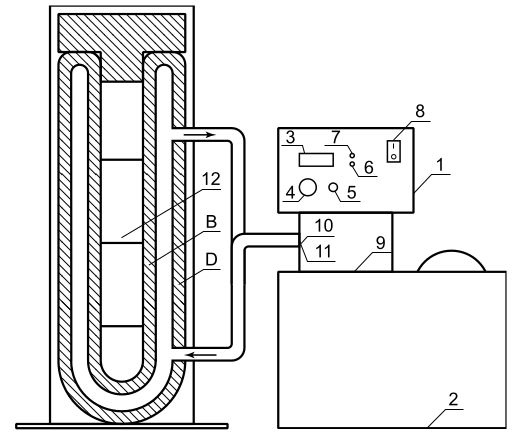
\includegraphics[scale=0.5]{asd.png}
\end{figure}
\section{Теоретическая часть}
Рассмотрим свободное падение шарика в вязкой жидкости. На
шарик действуют три силы: сила тяжести, архимедова сила и сила
вязкости, зависящая от скорости.

Найдем уравнение движения шарика в жидкости. По второму закону Ньютона:
\[
    Vg(\rho - \rho_{\textit{ж}}) - 6 \pi \eta rv = V \rho \frac{dV}{dt}
\]
Решая это уравнение, найдём:
\[
    v(t) = v_{\textit{уст}} - [v_{\textit{уст}}- v(0)]e^{\frac{-t}{\tau}}
\]\\
\[
    v_{\textit{уст}} = \frac{ Vg(\rho - \rho_{\textit{ж}})}{6 \pi \eta rv} = \frac{2}{9} \ gr^2\ \frac{\rho - \rho_{\textit{ж}}}{\eta}
\]\\
\begin{equation}
    \eta = \frac{2}{9} \ gr^2\ \frac{\rho - \rho_{\textit{ж}}}{v_{\textit{уст}}}
\end{equation}




\section{Обработка результатов измерений:}
\[
\begin{tabular}{|c|c|c|c|c|c|c|}
\hline   $\rho_{\textit{стекла}}$ & $\rho_{\textit{стали}}$ & $L_0$ & $L_1$ & $L_2$ & $d_{\textit{тр}}$ \\
\hline   $2.5 \frac{\textit{г}}{\textit{см}^3}$ & $7.8 \frac{\textit{г}}{\textit{см}^3}$ & $2.5 \pm 0.05 \textit{см}$ & $10.0 \pm 0.05 \textit{см}$ & $10.0 \pm 0.05 \textit{см}$ & $3.0 \pm 0.05 \textit{см}$ \\ 
\hline
\end{tabular}
\] 
\[
\begin{tabular}{|c|c|c|c|c|}
\hline   $T_1$ & $T_2$ & $T_3$ & $T_4$ & $T_5$ \\
\hline  $293.0 \pm 0.3\ \text{К}$ & $303.0 \pm 0.3\ \text{К}$ & $313.0 \pm 0.3\ \text{К}$ & $323.0 \pm 0.3\ \text{К}$ & $333.0 \pm 0.3\ \text{K}$ \\
\hline
\end{tabular}
\] \\
\[\begin{tabular}{|c|c|c|c|c|}
\hline  $T_1$  & 1 стекл. & 2 стекл. & 1 сталь. & 2 сталь. \\
\hline  $d$, мм & 2.10 & 2.20 & 0.85 & 0.80 \\
\hline  $t$, с & 4.81 & 4.61 & 5.30 & 6.10 \\
\hline $t_1$, с & 17.13 & 17.15 & 19.05 & 20.36 \\
\hline $t_2$, с & 17.45 & 17.13 & 18.83 & 20.29 \\
\hline
\end{tabular}
\]
\[
\begin{tabular}{|c|c|c|c|c|}
\hline  $T_2$  & 1 стекл. & 2 стекл. & 1 сталь. & 2 сталь. \\
\hline  $d$, мм & 2.10 & 2.10 & 0.70 & 0.75 \\
\hline  $t$, с & 2.60 & 2.65 & 3.96 & 3.60 \\
\hline $t_1$, с & 8.72 & 8.54 & 15.82 & 13.33 \\
\hline $t_2$, с & 8.64 & 8.73 & 15.64 & 13.79 \\
\hline
\end{tabular} 
\]
\[
\begin{tabular}{|c|c|c|c|c|}
\hline  $T_3$  & 1 стекл. & 2 стекл. & 1 сталь. & 2 сталь. \\
\hline  $d$, мм & 2.05 & 2.05 & 0.80 & 0.80 \\
\hline  $t$, с & 1.29 & 1.31 & 1.48 & 1.58 \\
\hline $t_1$, с & 5.29 & 5.29 & 5.03 & 5.33 \\
\hline $t_2$, с & 5.43 & 5.47 & 5.19 & 5.39 \\
\hline
\end{tabular} 
\]
\[\begin{tabular}{|c|c|c|c|c|}
\hline  $T_4$  & 1 стекл. & 2 стекл. & 1 сталь. & 2 сталь. \\
\hline  $d$, мм & 2.05 & 2.10 & 0.70 & 0.75 \\
\hline  $t$, с & 0.83 & 0.76 & 0.70 & 0.96 \\
\hline $t_1$, с & 2.70 & 2.69 & 3.45 & 3.39 \\
\hline $t_2$, с & 2.83 & 2.80 & 3.73 & 3.73 \\
\hline
\end{tabular} 
\]
\[
\begin{tabular}{|c|c|c|c|c|}
\hline  $T_5$  & 1 стекл. & 2 стекл. & 1 сталь. & 2 сталь. \\
\hline  $d$, мм & 2.00 & 2.05 & 0.75 & 0.85 \\
\hline  $t$, с & 0.45 & 0.53 & 0.58 & 0.46 \\
\hline $t_1$, с & 1.54 & 1.72 & 2.23 & 1.67 \\
\hline $t_2$, с & 1.89 & 1.90 & 2.27 & 1.96 \\
\hline
\end{tabular} 
\]




Вычислим значения $\eta$ для каждого опыта по формуле (1):
\[
 [\eta] =  \textit{Па} \cdot c
\]
\[
\begin{tabular}{|c|c|c|c|c|}
\hline   $\eta_1$ & $\eta_2$ & $\eta_3$ & $\eta_4$ & $\eta_5$ \\
\hline  $2.04 \pm 0.1224$ & $1.04 \pm 0.0624$ & $0.61 \pm 0.0366$ & $0.31 \pm 0.0186$ & $0.18 \pm 0.0108$ \\
\hline
\end{tabular}
\]
Оценим время релаксации $\tau$ и путь релаксации $S$ по формуле:
\[
\tau = \frac{V\rho}{6\pi\eta r} = \frac{2}{9} \frac{r^2\rho}{\eta}, \hspace{40pt} S=v_{\textit{уст}} \cdot t
\]
\[
\begin{tabular}{|c|c|c|c|c|}
\hline   $\tau_1$ & $\tau_2$ & $\tau_3$ & $\tau_4$ & $\tau_5$ \\
\hline   $0.0012\ c$ & $0.0024\ c$ & $0.0038\ c$ & $0.072\ c$ & $0.0075$\ c\\
\hline
\end{tabular}
\]
\[
\begin{tabular}{|c|c|c|c|c|}
\hline   $S_1$ & $S_2$ & $S_3$ & $S_4$ & $S_5$ \\
\hline   $7.05\cdot 10^{-3}\ \text{мм}$ & $2.7 \cdot 10^{-2}\ \text{мм}$ & $7.2 \cdot 10^{-2}\ \text{мм}$ & $0.2\ \text{мм}$ & $0.5\ \text{мм}$\\
\hline
\end{tabular}
\]
Путь релаксации $S \ll L_0 \Rightarrow$ скорость после $L_0$ является постоянной.
\newpage


Построим график зависимости $\ln \eta$ от $\frac{1}{T}$\,:

\begin{figure}[h!]
	\center
	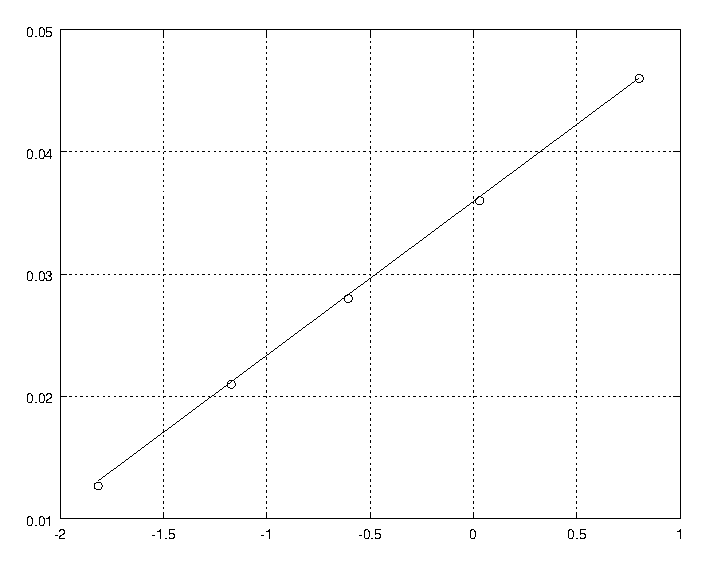
\includegraphics[scale=0.6]{latex3.png}
\end{figure}
Угловой коэффициент наклона равен $a = \frac{d\ln\eta}{d(1/T)} = 75.628$
\\
Оценим погрешности:
\[
    \varepsilon_L = \frac{\Delta_L}{L} = 0.02
\]
\[
    \varepsilon_T = \frac{\Delta_T}{T} = 0.02
\]
\[
    \varepsilon_r = \frac{\Delta_r}{r} = 0.048
\]
\[
    \varepsilon_{\eta} = 0.0634
\]
\[
	\varepsilon_W = 0.08452
\]

Найдём энергию активации молекулы: 
\[
W = k \frac{d\ln\eta}{d(1/T)} = (1.04416 \pm 0.08825)\,\cdot 10^{-21}\ \text{Дж}
\]

Посчитаем число Рейнольдса:
\[
\begin{tabular}{|c|c|c|c|c|}
\hline   $Re_1$ & $Re_2$ & $Re_3$ & $Re_4$ & $Re_5$ \\
\hline   $0.008$ & $0.032$ & $0.08$ & $0.03$ & $0.07$ \\
\hline
\end{tabular}
\]
Каждое значение числа Рейнольдса $Re < 0.5 \Rightarrow$ обтекание можно считать ламинарным.\\

\end{document}
